%%%%%%%%%%%%%%%%%%%%%%%%%%%%%%%%%%%%%%%%%%%%%%%%%%%%%%%%%%%%%%%
%%%  NEG 
%%%%%%%%%%%%%%%%%%%%%%%%%%%%%%%%%%%%%%%%%%%%%%%%%%%%%%%%%%%%%%%

% For submission redefine \rmrk \hrefl \hidea

\documentclass[aps,pre,floats,floatfix,twocolumn]{revtex4-1}
%\documentclass[fleqn,10pt]{wlscirep}

% special 
\usepackage{ifthen}
\usepackage{ifpdf}
\usepackage{color}

\ifpdf
\usepackage{graphicx}
\usepackage{epstopdf}
\else
\usepackage{graphicx}
\usepackage{epsfig}
\fi
\graphicspath{{./Figs_SBM_jpg/}{./}}
\graphicspath{{/Users/danielhurowitz/PROJ/NHR/Figs/}{/Users/danielhurowitz/PROJ/NEG/Figs/}{./}{../}}

% fonts
\usepackage{latexsym}
\usepackage{amsmath}
\usepackage{amssymb}
\usepackage{bm}
\usepackage{wasysym}

\usepackage{mathptmx}
\DeclareSymbolFont{epsilon}{OML}{ntxmi}{m}{it}
\DeclareMathSymbol{\epsilon}{\mathord}{epsilon}{"0F}

\usepackage{hyperref}

% Standard symbols 
\newcommand{\sinc}{\mbox{sinc}}
\newcommand{\const}{\mbox{const}}
\newcommand{\trc}{\mbox{trace}}
\newcommand{\intt}{\int\!\!\!\!\int }
\newcommand{\ointt}{\int\!\!\!\!\int\!\!\!\!\!\circ\ }
\newcommand{\ar}{\mathsf r}
\newcommand{\im}{\mbox{Im}}
\newcommand{\re}{\mbox{Re}}

% Special symbols
\newcommand{\mass}{\mathsf{m}} 
\newcommand{\Mass}{\mathsf{M}} 

% Math constractions
\newcommand{\tbox}[1]{\mbox{\tiny #1}}
\newcommand{\bmsf}[1]{\bm{\mathsf{#1}}} 
\newcommand{\amatrix}[1]{\begin{matrix} #1 \end{matrix}} 
\newcommand{\eexp}[1]{\mathrm{e}^{#1}}
\newcommand{\pd}[2]{\frac{\partial #1}{\partial #2}}
\newcommand{\bra}[1]{\left\langle #1 \right|}
\newcommand{\ket}[1]{\left| #1 \right\rangle}
\newcommand{\braket}[1]{ \left\langle #1 \right\rangle}
\newcommand{\Braket}[2]{ \left\langle #1 \middle| #2 \right\rangle}
\newcommand{\BraKet}[3]{ \left\langle #1 \middle| #2 \middle| #3 \right\rangle}
\newcommand{\avg}[1]{\left\langle #1 \right\rangle}
\newcommand{\ola}{\protect\overleftarrow}
\newcommand{\ora}{\protect\overrightarrow}

% Equations
\newcommand{\be}[1]{\begin{eqnarray}\ifthenelse{#1=-1}{\nonumber}{\ifthenelse{#1=0}{}{\label{e#1}}}}
\newcommand{\beq}{\begin{eqnarray}}
\newcommand{\eeq}{\end{eqnarray}} 

% Text arrangement
\newcommand{\hide}[1]{}

\newcommand{\Eq}[1]{\textcolor{blue}{{equation}\!~(\ref{#1})}} 
\newcommand{\Ap}[1]{\textcolor{blue}{{appendix}\!~(\ref{#1})}} 
\newcommand{\Sec}[1]{\textcolor{blue}{{section}\!~(\ref{#1})}} 
\newcommand{\Fig}[1]{\textcolor{blue}{Fig.}\!\!~\ref{#1}}
\newcommand{\sect}[1]{{\bf #1.-- }}
\newcommand{\drawline}{\begin{picture}(500,1)\line(1,0){500}\end{picture}}
\newcommand{\bitem}{$\bullet$ \ \ \ }
\newcommand{\Cn}[1]{\begin{center} #1 \end{center}}
%\renewcommand{\cite}[1]{\textcolor{blue}{[\onlinecite{#1}}]} %{[\onlinecite{#1}]} 



% temporary turn off figures
%\renewcommand{\includegraphics}[2][]{{\color{blue} \hspace{1cm} --FIGURE-- \hspace{1cm} }}

%\newcommand{\rmrk}[1]{{#1}}     %{\textcolor[rgb]{0.6,0,0.1}{#1}}
\newcommand{\rmrk}[1]{{\color[rgb]{0.6,0,0.1} #1}}
\newcommand{\hrefl}[1]    {\href{#1}{[link]}}
\newcommand{\hidea}[1]{}    %{{#1}}


%%%%%%%%%%%%%%%%%%%%%%%%%%%%%%%%%%%%%%%%%%%%%%%%%%%%%%%%%%%%%%%%%%%%%%%%%%%%%%%%%%%%%%%%%%
%%%%%%%%%%%%%%%%%%%%%%%%%%%%%%%%%%%%%%%%%%%%%%%%%%%%%%%%%%%%%%%%%%%%%%%%%%%%%%%%%%%%%%%%%%
\begin{document}
 
\title{Percolation, sliding, localization and relaxation in glassy circuits}

\author{DH and DC}

\affiliation{Department of Physics, Ben-Gurion University of the Negev, Beer-Sheva, Israel}

%%%%%%%%%%%%%%%%%%%%%%%%%%%%%%%%%%%%%%%%%%%%%%%%%%%%%%%%%%%%%%%%%%%%%%%%%%%%%%%%%%%%%%%%%%
%%%%%%%%%%%%%%%%%%%%%%%%%%%%%%%%%%%%%%%%%%%%%%%%%%%%%%%%%%%%%%%%%%%%%%%%%%%%%%%%%%%%%%%%%%

%\begin{abstract}
%\end{abstract}

\maketitle
%
%
%There is a recent interest in ``glassy" systems that have log-wide distribution of 
%relaxation rates. For example we note recent works regarding electron dynamics where 
%the effective model is essentially the same as {\em random walk in disordered lattice}. 
%In such type of model there is a percolation-related crossover to sub-diffusion (in one dimension), 
%or to variable-range-hopping type diffusion (in general). 
%This crossover is reflected in the spectral properties of the system.
%%
%The more general problem of {\em random walk in random environment}, 
%where transitions between sites are allowed to be asymmetric, 
%has been explored by Sinai, Derrida, and followers. 
%Focusing on one-dimensional systems, it turns out that 
%for any small amount of disorder an unbiased spreading 
%becomes sub-diffusive. For bias that exceeds a non-zero threshold there 
%is a {\em sliding transition}, and the drift velocity becomes non-zero.
%%
%Considering an $N$-site ring geometry, we ask what are the implications 
%of the percolation and of the sliding transitions on the relaxation modes 
%of such topologically closed system. A complementary question regarding  
%the ``delocalization" of eigenstates of non-Hermitian quantum Hamiltonians
%has been addressed by Hatano, Nelson, and followers. 
%We show below that for a conservative "random walk" dynamics 
%the implied spectral properties are dramatically different.
%  
  
  

There is recent interest in ``glassy" systems that have log-wide distribution of 
relaxation rates \cite{glass1}. For example we note recent works regarding electron dynamics where 
the effective model is essentially the same as a {\em random walk on a disordered lattice} \cite{ege,egt}. 
In such type of model there is a percolation-related crossover to sub-diffusion (in one dimension), 
or to variable-range-hopping type diffusion (in general) \cite{pts}. 
This crossover is reflected in the spectral properties of the system.
A similar point of view regarding percolation is the continuous time random walk (CTRW) with
a broad distribution of waiting times \cite{BouchaudReview}.


The more general problem of {\em random walk in random environment}, 
where transitions between sites are allowed to be asymmetric, 
has been explored by Sinai \cite{Sinai}, Derrida \cite{odh1}, and followers \cite{odh3,BouchaudReview}. 
Focusing on one-dimensional systems, it turns out that 
for any small amount of disorder an unbiased spreading 
becomes sub-diffusive. For bias that exceeds a non-zero threshold there 
is a {\em sliding transition}, and the drift velocity becomes non-zero.
This type of dynamics is relevant to studies in a biophysical context: pulling
pinned polymers, DNA denaturation \cite{DNA1, DNA2}, population biology \cite{popbio,popbio2}, and molecular motors \cite{brm1,brm2}. 
The bias in the case of depinning polymers and DNA denaturation is the pulling force.
In the case of population biology, it is the convective flow of bacteria relative to the nutrients and for molecular motors it is the affinity 
of the chemical cycle. 
The sliding transition is a major theme in the latter context.

Considering a finite system, the prototype being an $N$-site ring, one
asks what are the relaxation modes of such a topologically closed system. In the Brownian
motor context $N$ is the length of a cycle, i.e. the number of chemical reactions required to advance
the motor by one step. 
In the remaining examples, sites have a spatial context and the number of sites $N$ arises from the underlying lattice.

%Considering an $N$-site ring geometry, we ask what are the implications 
%of the percolation and of the sliding transitions on the relaxation modes 
%of such topologically closed system.
 A complementary question regarding  
the ``delocalization" of eigenstates of non-Hermitian quantum Hamiltonians
has been addressed by Hatano, Nelson, and followers \cite{Hatano1,Hatano2, Shnerb1},  originally in the context of vortex depinning in type II superconductors. In this case, the bias is the applied transverse magnetic field and $N$ is the number of defects to which the magnetic vortex can pin.
Their main achievement is the realization that the complex spectrum of the non-Hermitian hamiltonian 
can be deduced from the real spectrum of an associated Hermitian hamiltonian. 
Various improvements on the method and ensuing analytical results were obtained.
For example, the complex spectrum in the thermodynamic limit was found in \cite{Brouwer}.
An equation for the curve in the complex plane on which the eigenvalues are located and the density of states was found in \cite{Goldsheid}.
Results for special models of one impurity and one way dynamics (maximally asymmetric transition rates) were obtained in \cite{Zee}.
%
%The physical phenomena that inspired this line of work is vortex depinning in type II superconductors \cite{Hatano1,Hatano2}, yet parallels to non quantum systems were drawn. Such systems include pulling pinned polymers, DNA denaturation \cite{DNA1,DNA2} and non conservative population biology \cite{popbio,popbio2}.

We show below that for a conservative "random walk" dynamics 
the implied spectral properties are dramatically different.
%  
Notable "conservative random walkers" are Brownian motors. For example, molecular motors on heterogeneous tracks, such as DNA or RNA. In \cite{brm1,brm2} non conservative motors are considered. It was found that under an external force and strong disorder, the motor will become localized at preferred positions yet near the stall force, localization occurs for any amount of disorder. These results were obtained by observing the numerically obtained spectrum. 

% In which case, they do make a connection with Derrida. They study the complexity vs. disorder in the detachment rate. 
%For $\mu>1 $, for weak disorder the spectrum is complex, for strong disorder there are real eigenvalues. 
%Form $\mu<1$, there are real eigenvalues even for very small disorder.

%%%%%%%%%%%%%%%%%%%%%%%%%%%%%%%%%%%%%%%%%%%%%%%%%%%%%%%%%%%%%%%%%%%%%%%%%%%%%%%%%%%%%%%%%%%%%%%%%%%%%%%%%%%%%%%%%%%%
\begin{figure}
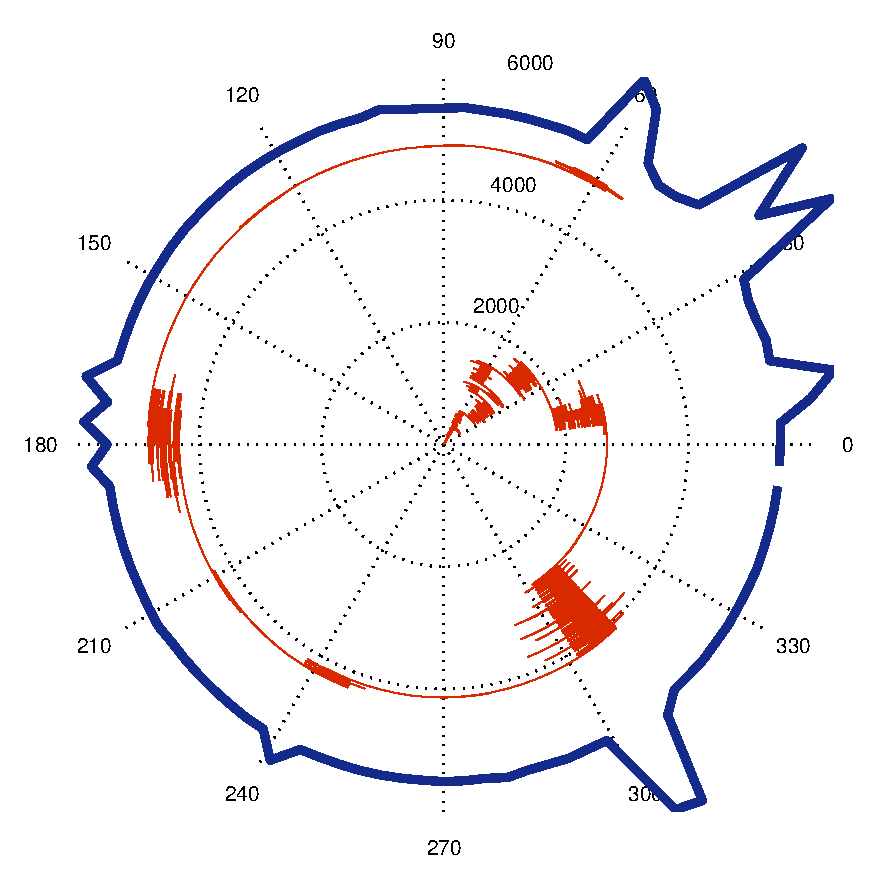
\includegraphics[height=6.5cm]{/Figs/polar_1_a.eps}
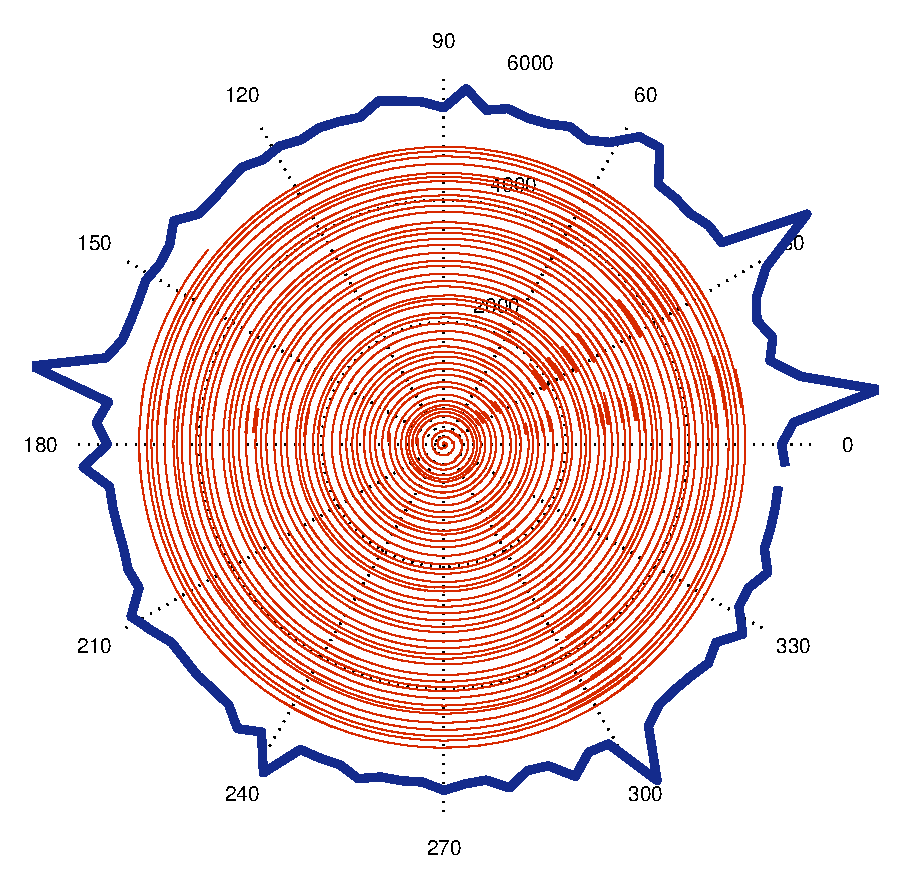
\includegraphics[height=6.5cm]{/Figs/polar_2_a.eps}
\caption{
Simulated trajectory of a particle on a disordered ring. The radial direction is time and the angle is the position. 
For small $s$ (top panel) the dynamics is overdamped, while for large $s$ (bottom panel) the dynamics is under damped. 
The thick line on the edge of the circle is the steady state distribution (See \Ap{Ap12}). For this figure there are $N=100$ sites, $\sigma=5$ and $s=0.88, \ 2.97$.
%Each panel shows several trajectories with the particle at randomly selected initial positions.
}
\label{traj}
\end{figure}

\begin{figure}
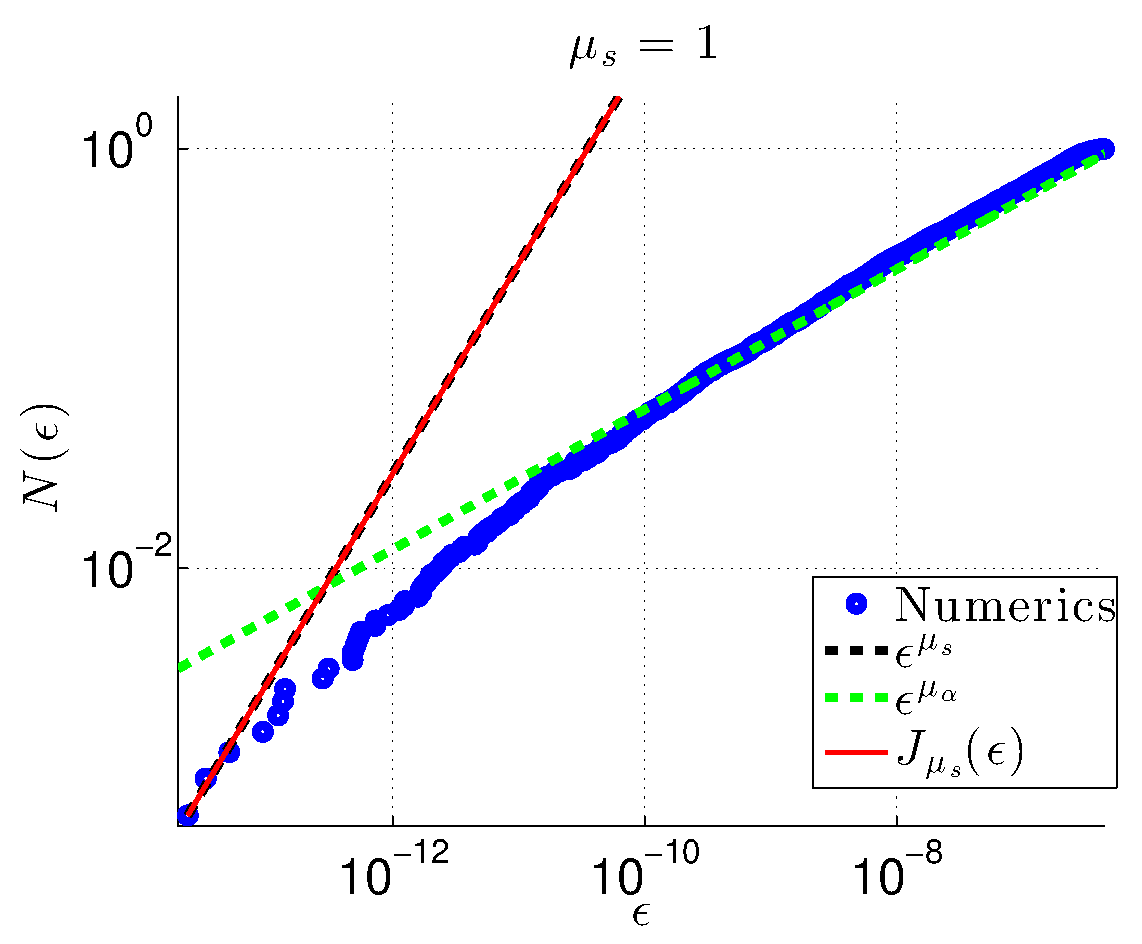
\includegraphics[height=5cm]{/Figs/N_E_1_1_french}
\caption{The integrated density of the $\epsilon_k$ for a ring with ${N=3000}$ sites. The
system is characterized by a percolation exponent ${\mu_{\alpha} = 1/3}$ and a scaled affinity ${\mu_s = 1}$.
 The width of the stochastic-field distribution is $\sigma=2$. 
 The blue points are are results of numerical diagonalization. 
 There is a crossover from density that corresponds to $\mu_s$ (dashed black line) to density that corresponds to $\mu_{\alpha}$ (dashed
green line). 
For small $\epsilon$  the result of \cite{odh3} (thin red line) coincides with the power law behavior that we assumed.
}
\label{fig2}
\end{figure}


\begin{figure*}
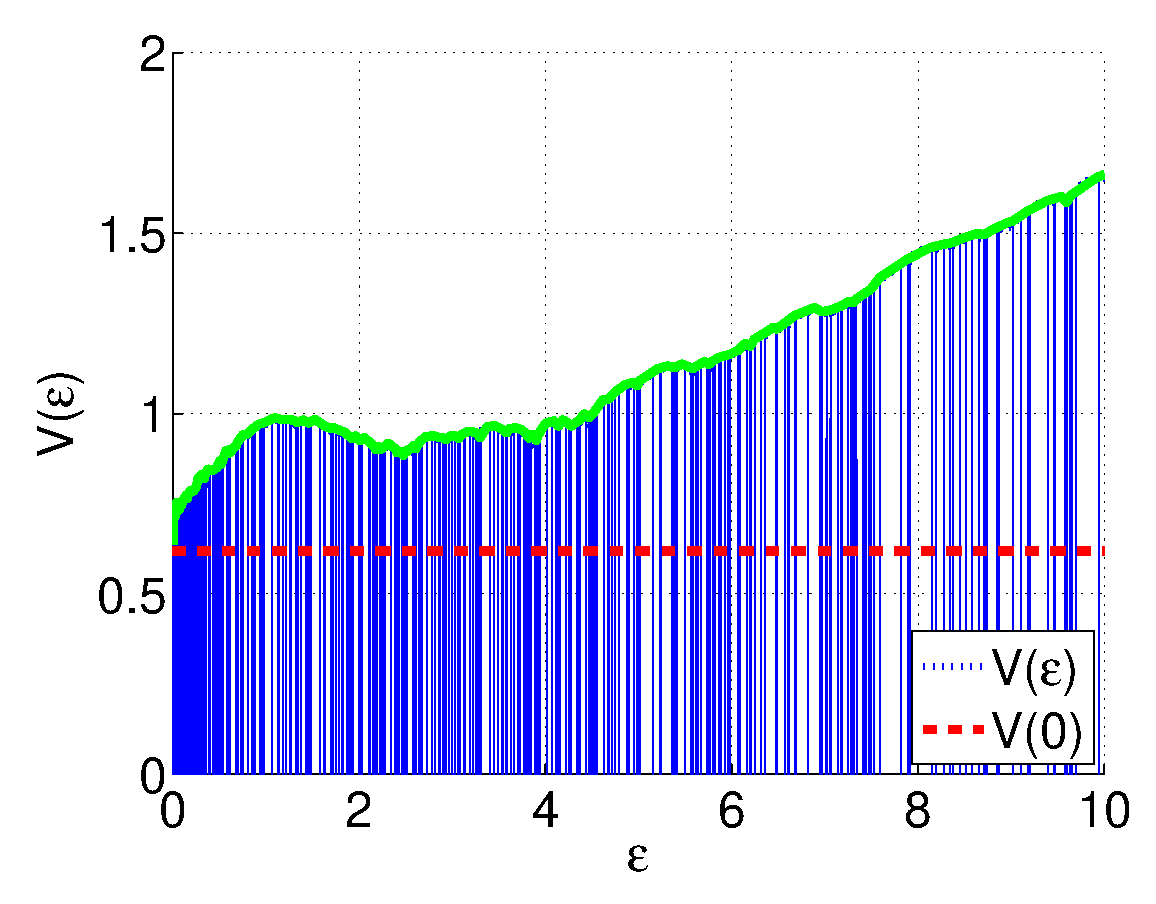
\includegraphics[height=4.5cm]{/Figs/V_E_1_2.eps}
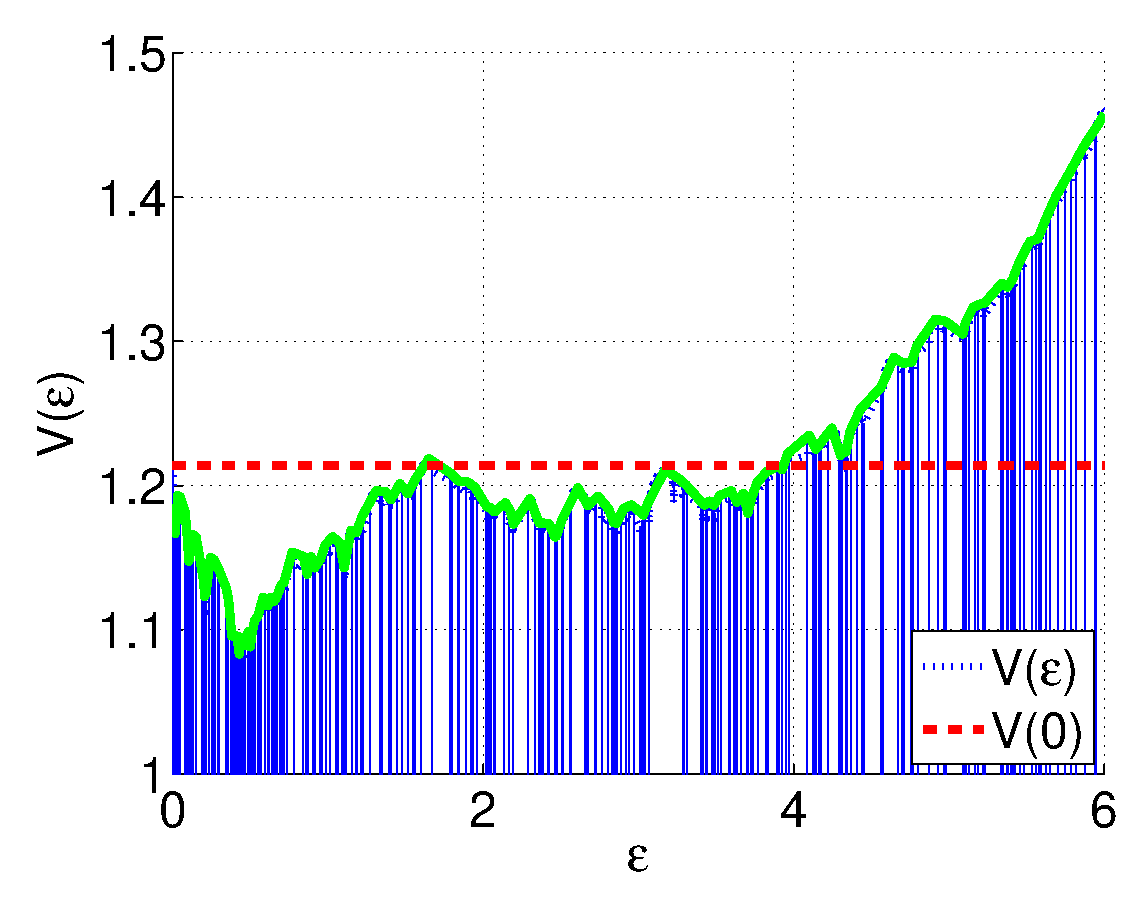
\includegraphics[height=4.5cm]{/Figs/V_E_1.eps}
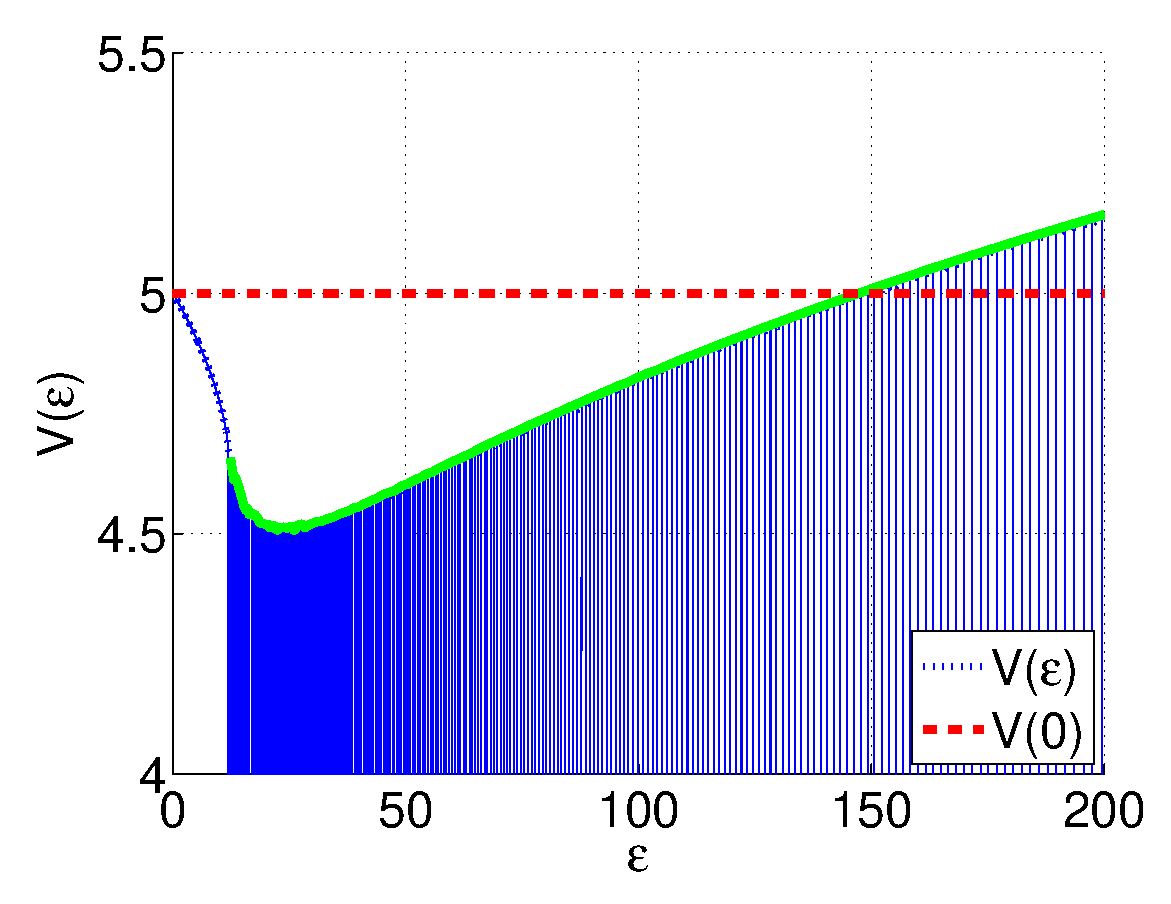
\includegraphics[height=4.5cm]{/Figs/V_E_2.eps}

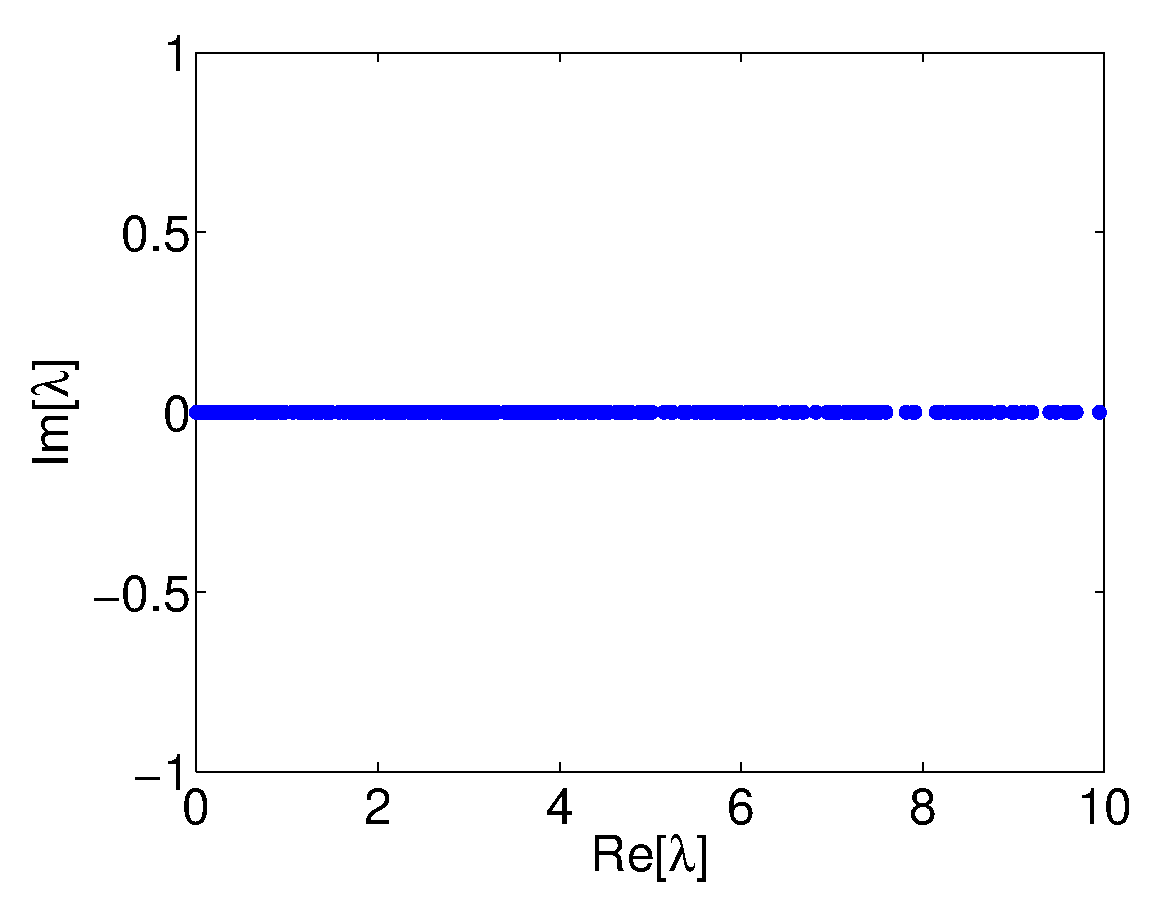
\includegraphics[height=4.5cm]{/Figs/spectrum_1_2.eps}
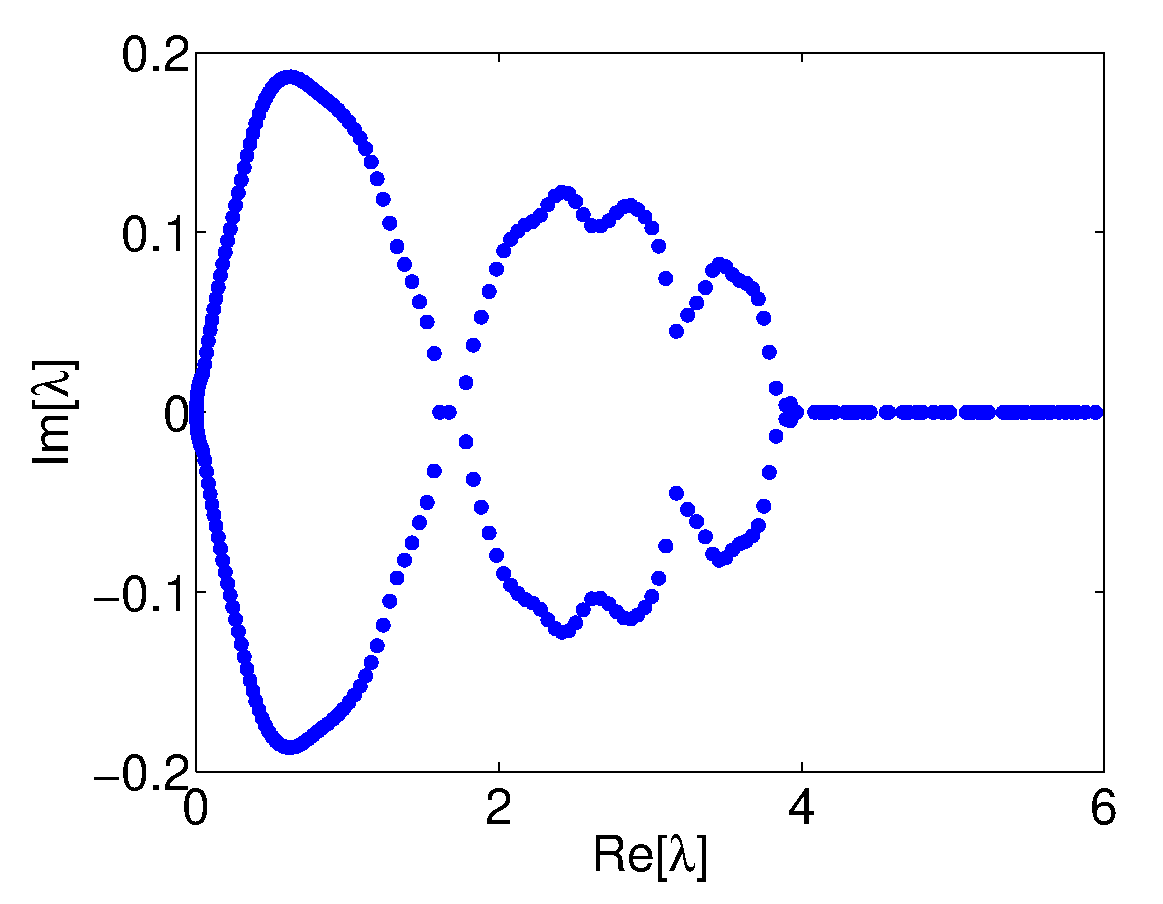
\includegraphics[height=4.5cm]{/Figs/spectrum_1.eps}
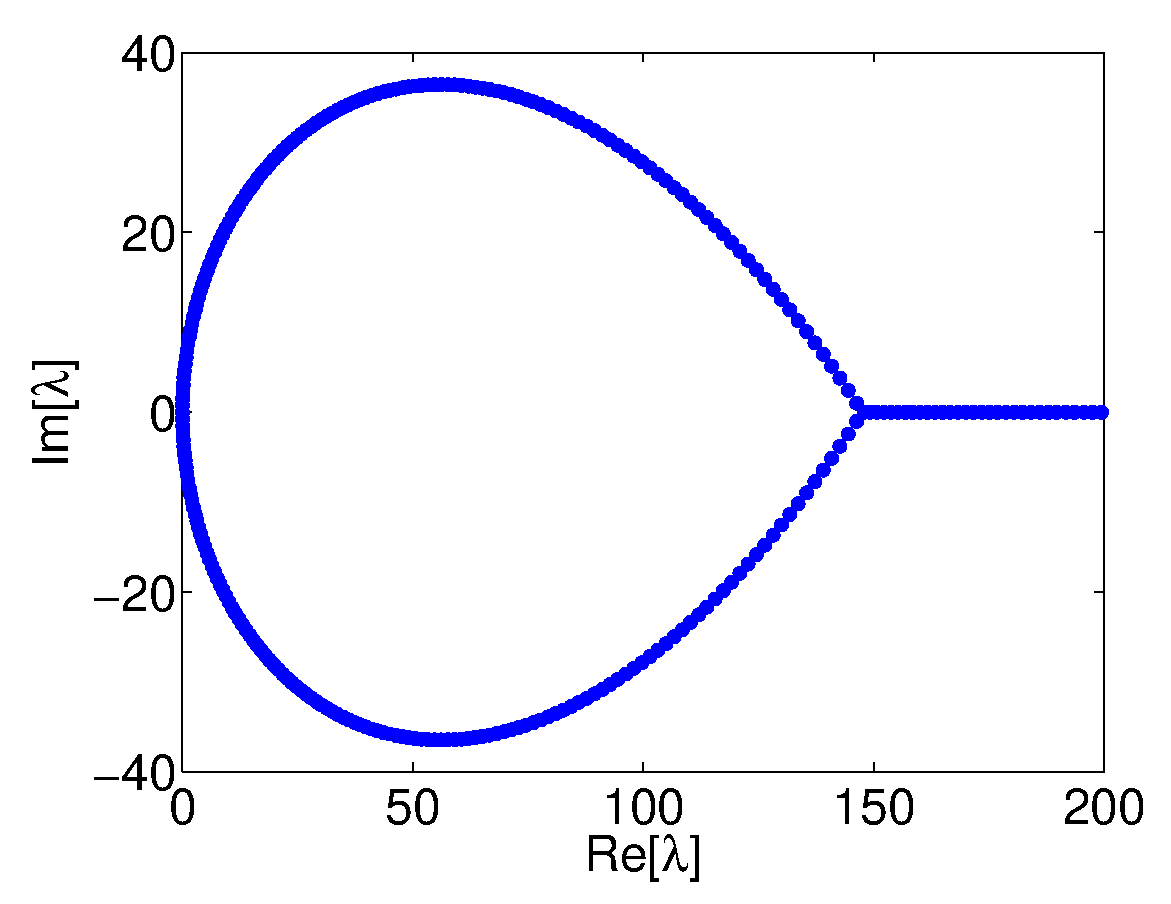
\includegraphics[height=4.5cm]{/Figs/spectrum_2.eps}
\caption{
Illustrating the route to complexity. The top row shows 
the electrostatic potential $V(\epsilon)$ along the real axis and the bottom row shows the associated spectrum in the complex plane. 
Here $N=500$, $\sigma = 5$, and (from left to right) $s=1.24, \ 2.43,\ 10$. For these parameters the threshold values are $s_{1/2}=1.77, \ s_1=2.7$ and $s_{\infty}=5$.
In the left hand column $s<s_{1/2}$ and the spectrum is real.
In the middle column $s_{1/2} <s <s_{\infty}$ and there is an interesting scenario of a mixed spectrum, where there might be several complex bubbles separated by real segments. 
In the right hand column  $s>s_{\infty}$ and the real spectrum has a gap (beginning with the first oscillation), but the complex spectrum does not (see also \Fig{figWeak}). 
Also, the spectrum is a fully developed complex bubble, where the bottom of the band is delocalized (underdamped modes) and the rest of the band 
is localized (or overdamped).
}
\label{f2}
\end{figure*}


\begin{figure}
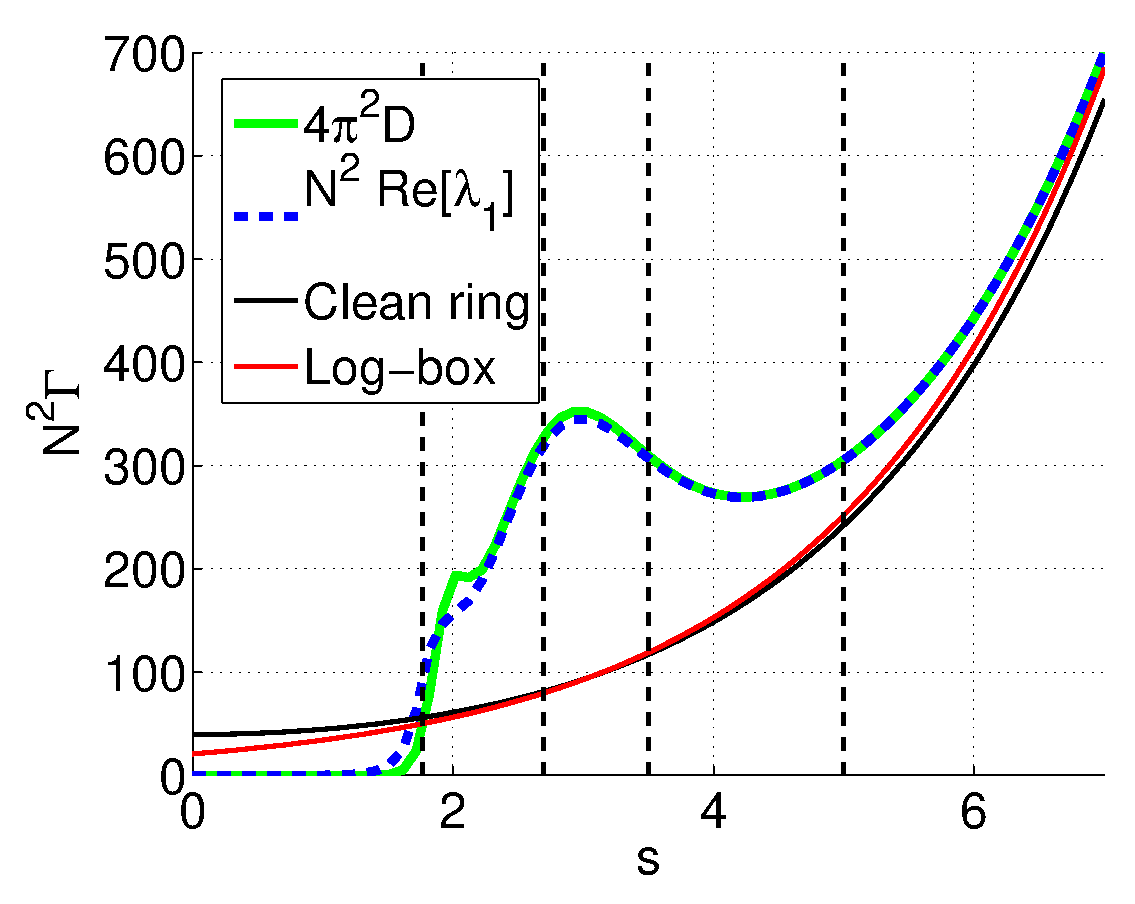
\includegraphics[height=6cm]{/Figs/gap_D_sigma5_N_1000.eps}
\caption{
The relaxation rate $\Gamma = \text{Re}[\lambda_1]$ versus the affinity $s$ for $N = 1000$ sites $\sigma = 5$. The non monotonic dashed blue line has been obtained via numerical diagonalization, whereas the solid green was obtained by calculating the diffusion coefficient as in \cite{nes}.
The monotonic lines correspond to the limits of
clean ring (\Eq{e13}, black) and $s>s_{\infty}$  (\Eq{e52}, red). The vertical dashed lines are the affinities 
$s_{\mu}$ that are associated with
the scaled values $\mu= 1/2, \ 1, \ 2, \ \infty$ (from left to right).}
%
%
%The real part of the gap of the complex spectrum $\Gamma = \text{Re}[\lambda_1]$ vs. $s$ for $N=1000$ sites and log-box field disorder with $\sigma=5$.
%The non monotonic dashed blue line was obtained by numerically diagonalization, 
%whereasthe solid green was obtained by calculating the diffusion coefficient as in \cite{nes}.
%The monotonic lines correspond to the limits if a clean ring \Eq{e13} (black) and $s>s_{\infty}$, \Eq{e52} (red).
%The vertical dashed lines from left to right are $s_{1/2},\  s_{1},\ s_{2}$ and $s_{\infty}$.    }t
\label{f1}
\end{figure}
%
\begin{figure}[h!]
 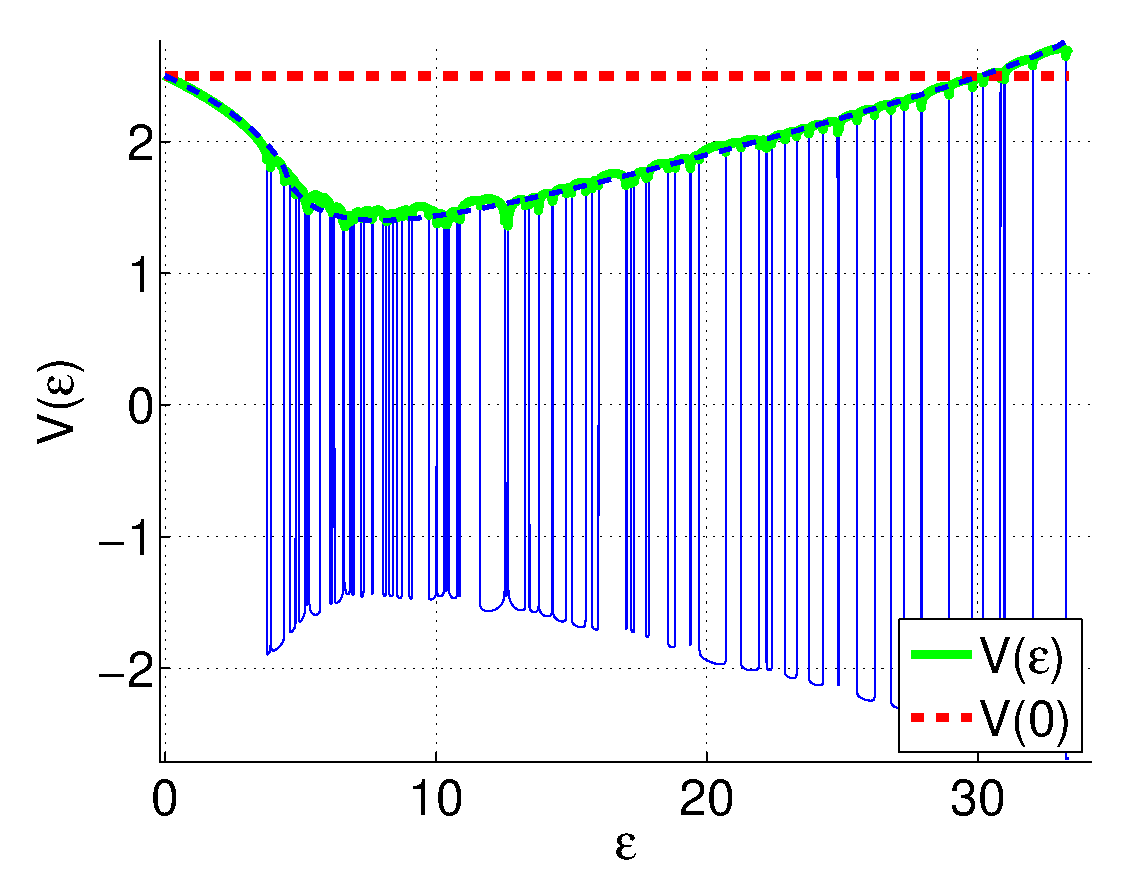
\includegraphics[width=6.2cm]{/Figs/V_E_s_inf}
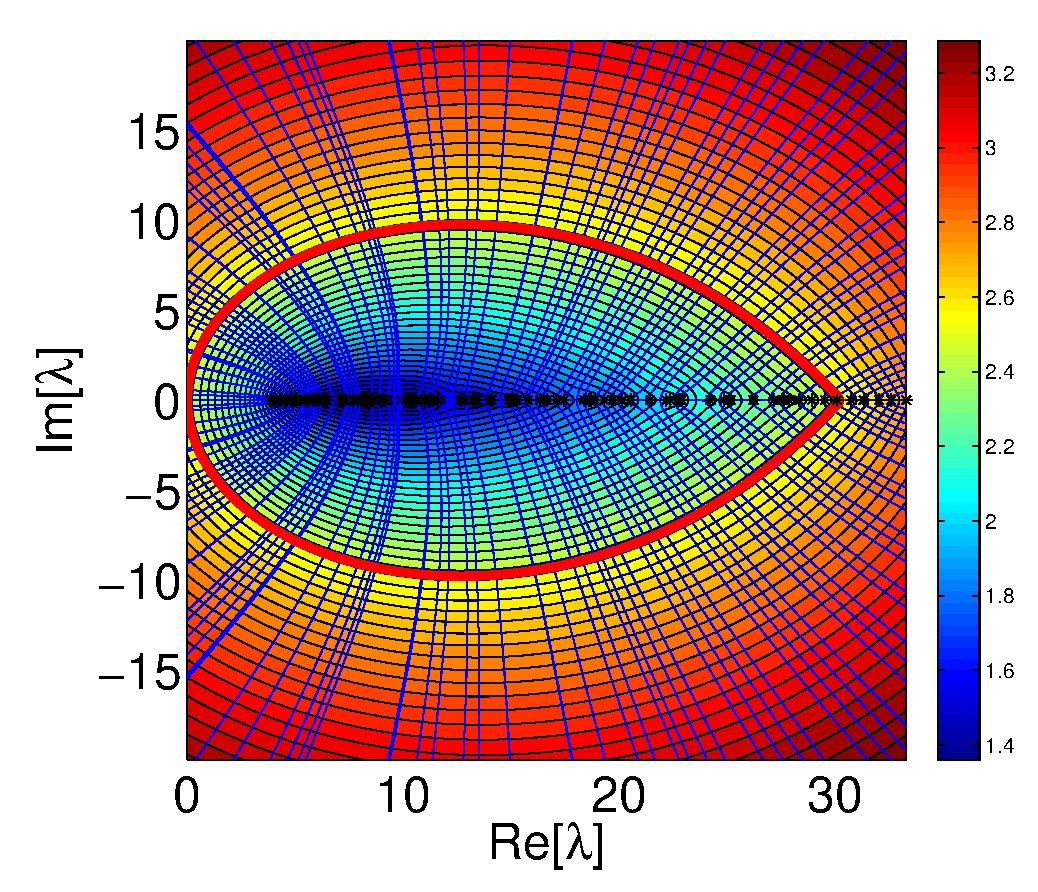
\includegraphics[width=7.5cm]{/Figs/electrostatics_large_S}
 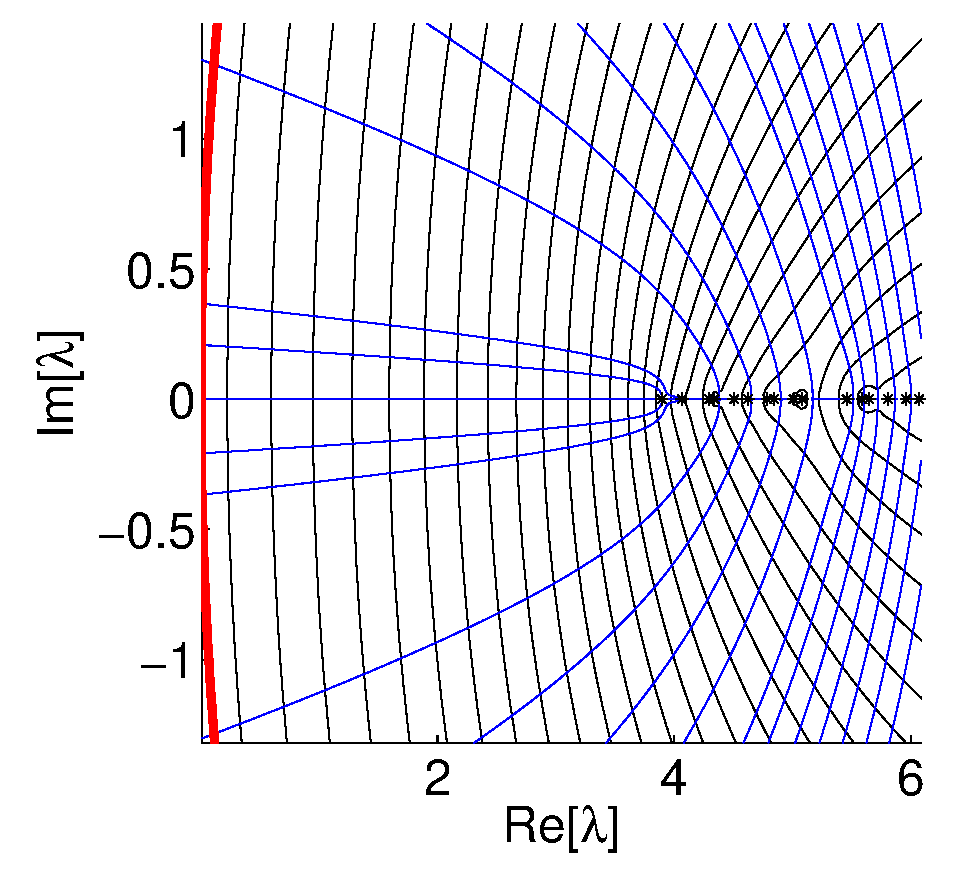
\includegraphics[width=7.5cm]{/Figs/electrostatics_large_S_zoom}

\caption{ {\bf Top panel}: The electrostatic potential $V(\epsilon)$ along the real axis. 
%The green points are the result of numerical diagonalization,
 The dashed blue line is the analytical result assuming $\rho=N(\sigma x)^{-1}$, \Eq{e43}. 
The stars 
indicate the position of the "charges", which are the eigenvalues of the associated Hermitian matrix, $\varepsilon_j$.
{\bf Middle panel}: 
The �electrostatic potential� $\Psi(z)$ of \Eq{e22}. Here we consider a ring with $N=100$
sites, $\sigma=2$ and $s=5$. The complex $\lambda_k$ spectrum is obtained by looking for the intersections of the field lineswith the red thick equipotential line $V(z)=V(0,0)$ that goes through the origin. 
%
{\bf Bottom panel}: Zoom. 
Note that the complex spectrum unlike the real spectrum does not have a gap.
%
%The red line is the equipotential line $V(\lambda) = V(0)$.
%The gap in the spectrum of $\bm{H}$  (black stars) is large, 
%but the real gap in the complex spectrum, (intersection
%of the contour $V=V(0)$and the first field line) diminishes as $1/N^2$.
%Here $N=100$ sites, $\sigma=2$ and $s=5$.
}
\label{figWeak}
\end{figure}
%%%%%%%%%%%%%%%%%%%%%%%%%
\begin{figure}[h]
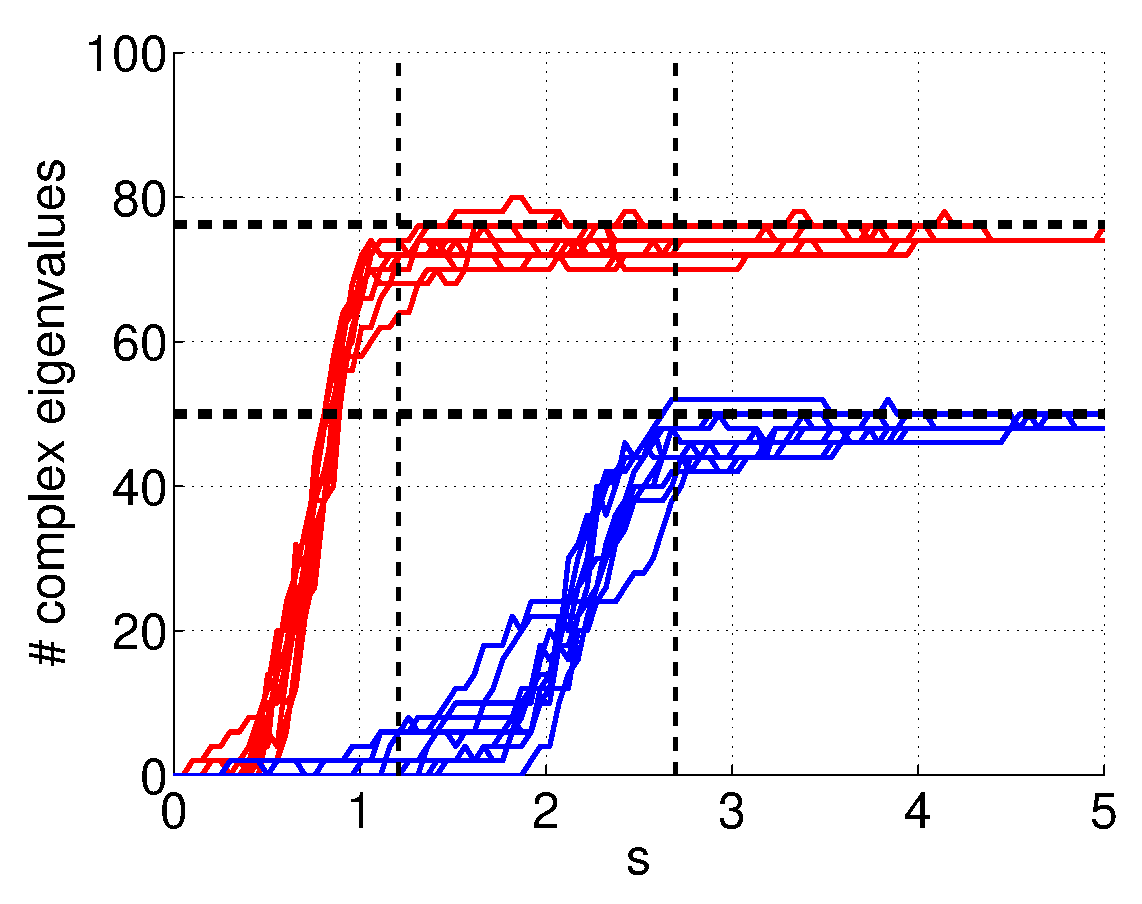
\includegraphics[height=5.4cm]{/Figs/numComplex_100}
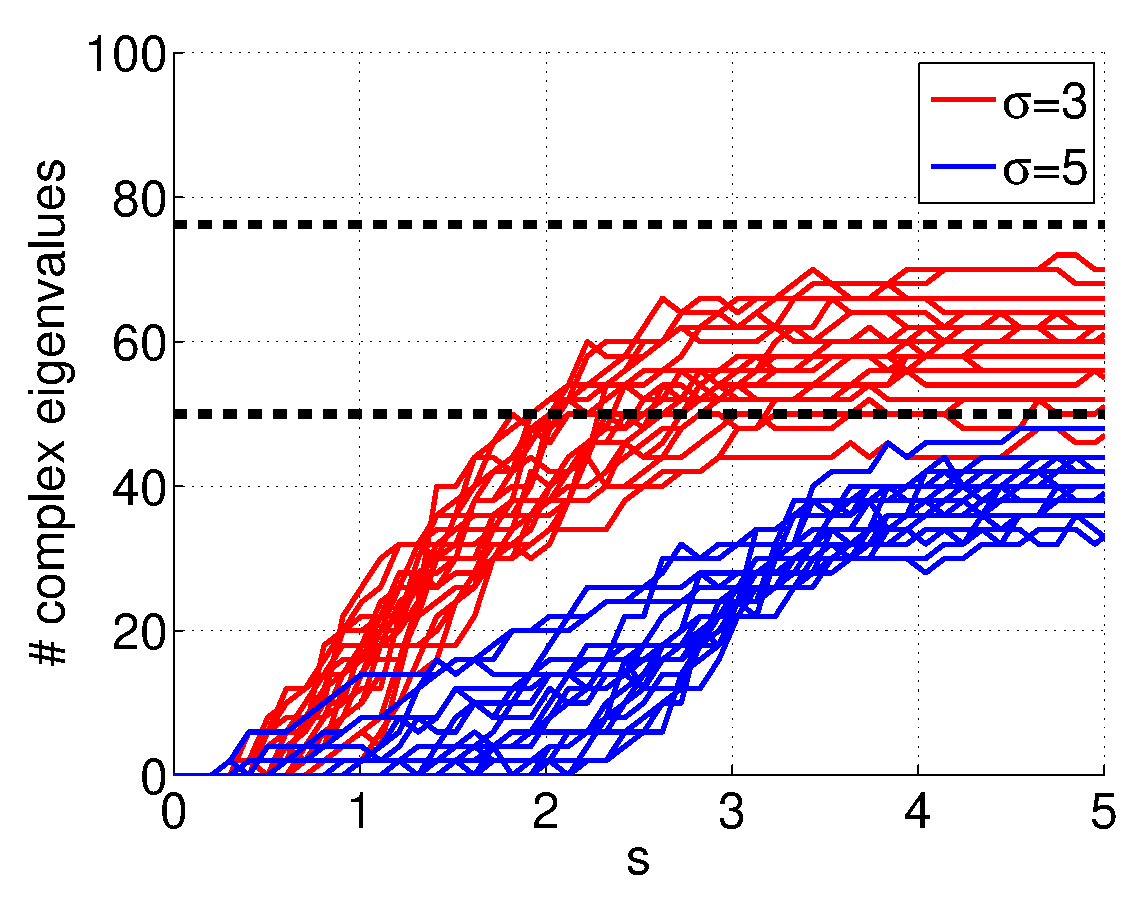
\includegraphics[height=5.4cm]{/Figs/numComplex_100_alpha}
%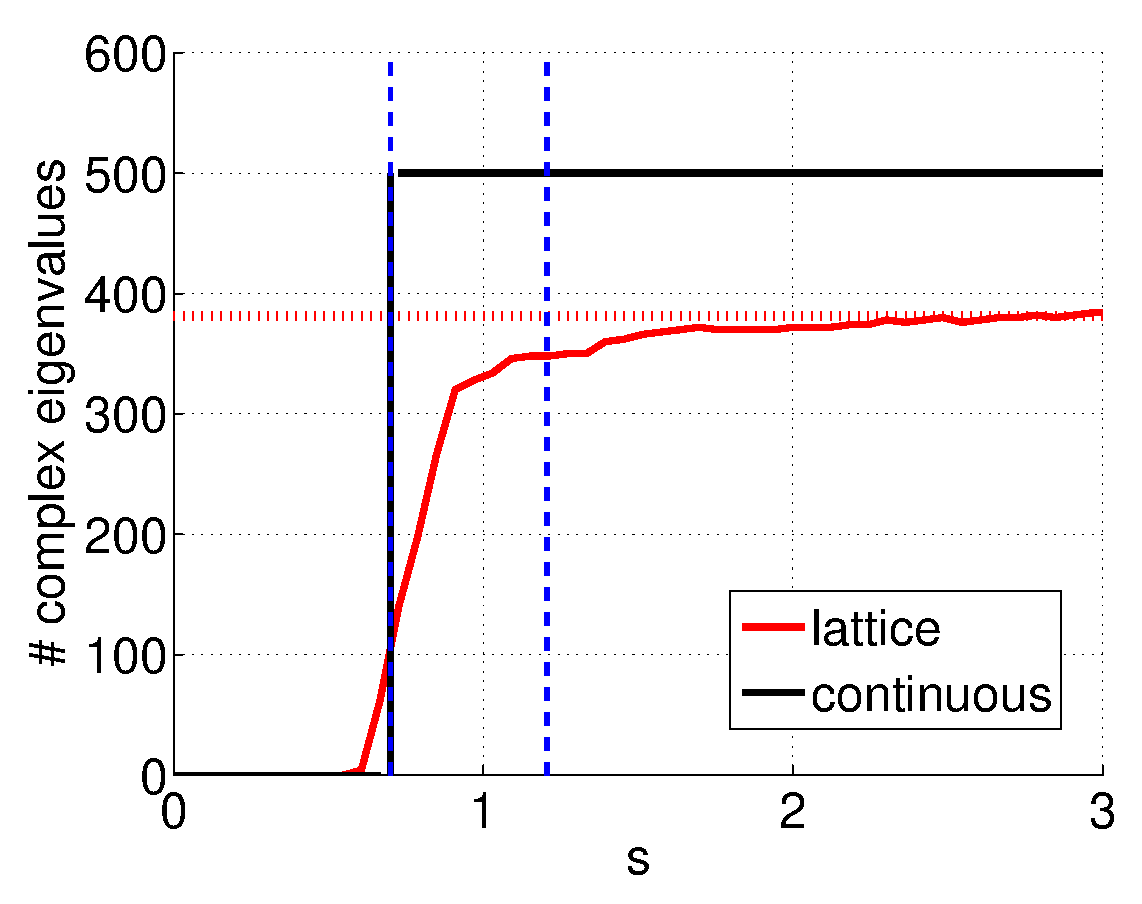
\includegraphics[height=5cm]{/Figs/numComplex_500}
\caption{
We count the number of complex eigenvalues
for a ring with $N=100$ sites, for various values of the affinity $s$. Each red line corresponds to a different
realization of field disorder with $\sigma=3$ (red) and $\sigma = 5$ (blue). 
The black vertical lines are at values of $s_1(\sigma)$
at which the sliding transition occurs. We see that the asymptotic fraction of complex eigenvalues saturates,
which is quite different from what is known for non-conservative non-Hermitian matrices. The horizontal
dashed line are analytical estimates of \Eq{e101}. 
If the lattice were continuous and the disorder white noise, the number of complex eigenvalues would 
go from 0 to 100 at $s=s_{1/2}$.
On the bottom panel $\alpha=0.9$, the crossover is blurred and the saturation value is lower (the horizontal lines are calculated for $\alpha=\infty$).
}
\label{figCplxSat}
\end{figure}

\clearpage

\bibliography{neg_bib.bib}{}

\end{document}
%%%%%%%%%%%%%%%%%%%%%%%%%%%%%%%%%%%%%%%%%%%%%%%%%%%%%%%%%%%%%%%%%%%%%%%%%%
%%%%%%%%%%%%%%%%%%%%%%%%%%%%%%%%%%%%%%%%%%%%%%%%%%%%%%%%%%%%%%%%%%%%%%%%%%


